\documentclass{beamer}
\usetheme{Berlin}
\usepackage[latin1]{inputenc}
\usepackage{graphicx}
\usepackage{alltt}
\usepackage[spanish]{babel}
\title{Informe de Tarea 2 - Juego Skynet}
\author{Francisco Ar\'evalo\\
  \texttt{francisco.arevalod@alumnos.usm.cl}\\
  \texttt{http://github.com/farevalod/fisw-tarea2}\\
  \vspace{10mm}
  Departamento de Inform\'atica\\
  Universidad T\'ecnica Federico Santa Mar\'ia\\
  Santiago, Chile}
\date{\today}
\begin{document}
\maketitle
\tableofcontents
\section{Domain Model}
\begin{frame}
\begin{figure}[htb]
\centering
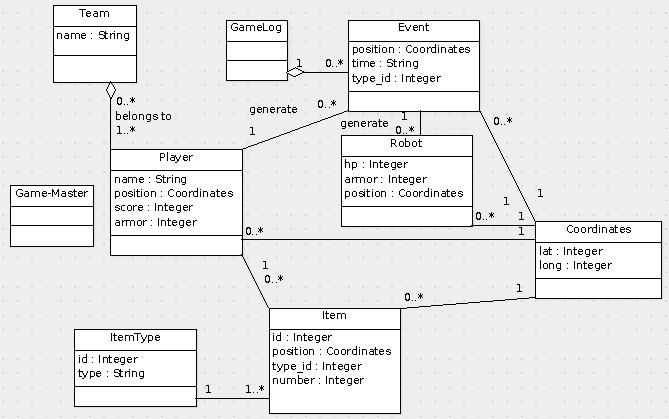
\includegraphics[scale=0.5]{domain-model}
\caption{Domain model displaying entities, attributes, relations and associations.}
\end{figure}
\subsection{Generated code from UML}
The code generated by the UML modeling tool can be browsed and downloaded from: 
\url{https://github.com/farevalod/fisw-tarea2}
\end{frame}
\section{Use Case}
\begin{frame}
\begin{figure}[htb]
\centering
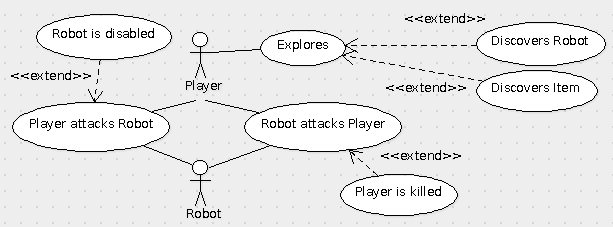
\includegraphics[scale=0.5]{basic-use-case}
\caption{Base and alternative use cases.}
\end{figure}
\end{frame}
\section{System Sequence Diagram}
\begin{frame}
\subsection{Basic Case}
\begin{figure}[htb]
\centering
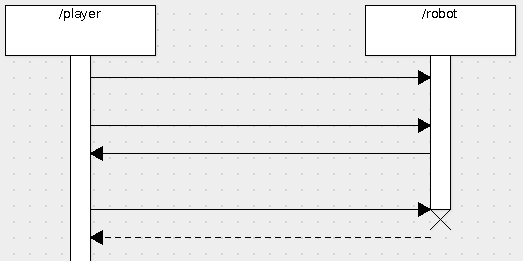
\includegraphics[scale=0.5]{basic-sequence}
\caption{Sequence diagram for common game loop.}
\end{figure}
\subsection{Alternative Cases}
\begin{figure}[htb]
\centering
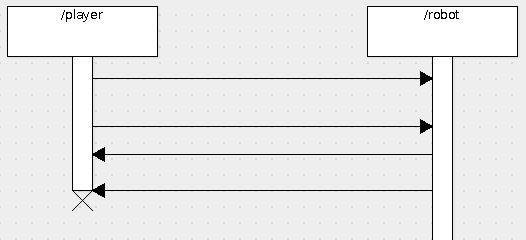
\includegraphics[scale=0.5]{player-dies-sequence}
\caption{Sequence diagram when player is killed.}
\end{figure}
\end{frame}
\end{document}
